\documentclass[main]{subfiles}

\begin{document}
\begin{lect}{2019-09-19}
		\begin{Reminder}
				\[D \text{ - мн-во}\]
				\begin{enumerate}
						\item $\displaystyle \dot{x} = X(t, x)$
						\item $\displaystyle (t_0, x_0) \in D$
				\end{enumerate}
		\end{Reminder}

		\begin{Definition}
				\[x = \varphi(t) \text{ - реш. задачи Коши } (1), (2), \q t \in <a, b>\]
				\[\text{единств. на } <a, b> \text{, если}\]
				\[\forall \text{ другое реш. } x = \psi(t) \text{ З.К. } (1),(2) \q t \in <a, b>\]
				\[\varphi(t) \equiv \varphi(t) \text{ на } <a, b>\]
		\end{Definition}

		\begin{theorem}
				В усл. теоремы Пеано, если решение $x = \varphi(t)$ - единств. на P
				\[(P = [t_0, t_0 + h]), \text{ то посл. ломанная Эйлера}\]
				\[\varphi_k(t) \us{k \to +\infty}{\os{p}{\rightrightarrows}} \varphi(t)\]
		\end{theorem}

		\begin{Proof}[От противного]
				\[\exists \mathcal{E} > 0: \forall k_0 \in \N \q \exists k > k_0, \exists t \in P :
				|\varphi_k(t) - \varphi(t)| \geq \mathcal{E}\]
				\[\Ra \exists \{k_j\}_{j = 1}^\infty, \q \{t_j\}_{j = 1}^\infty :
				k_{j + 1} > k_j \text{ и } |\varphi_{k_j}(t_j) - \varphi(t_j)| \geq \mathcal{E} \q (14) \]
				\[\{\varphi_{k_j}(t) \}_{j=1}^\infty \text{ - посл. Л.Э. } \Ra \text{ п/послед } \{\varphi_{k_{jm}}(t)\} _{m = 1}^\infty :\]
				\[\varphi_{k_{jm} } (t) \os{P}{\us{m \to  + \infty}{\rightrightarrows}} \psi(t) \]
				\[\Ra \forall \mathcal{E} > 0 \exists k_{j_0} : \forall k_{jm} > k_{j0} \q |\varphi_{k_{jm} } - \psi(t)| < \mathcal{E} \q(15)\]
				\[k_{jm} > k_{j_0}  \]
				\[|\varphi(t_{jm}) - \psi(t_{jm})| \geq |\underbracket{\varphi(t_{jm}) - \varphi_{kjm}(t_{jm} )}_{\geq \mathcal{E}} |
				- |\underbracket{\varphi_{kjm}(t_{jm}) - \psi(t_{jm})}_{< \mathcal{E}} | > 0\]
				\[\Ra \varphi(t_{jm}) \neq \psi(t_{jm}) \text{ - против. с единственностью } \varphi(t) \text{ на } P \]
		\end{Proof}

		\addcontentsline{toc}{subsection}{Теорема Пеано}
		\begin{Theorem} [Пеано]
				\[X \in C(G), \q \underbracket{G}_\text{обл} \subset \R^2\]
				\begin{enumerate}
						\item $\dot{x} = X(t, x)$
						\item $(t_0, x_0) \in G$
				\end{enumerate}
				\[\Ra \exists h > 0 : \text{ на } [t_0 - h, t_0 + h] \text{ опред. решение з. К } (1), (2)\]
				\[x = \varphi(t)\]
		\end{Theorem}

		\begin{Proof}
				\[\forall(t_0, x_0) \in G \q \exists a > 0, b > 0:\]
				\[D = \{(t, x) : |t - t_0| \leq a, |x - x_0| \leq b\} \subset G\]
				\[\Ra h = \min(a, \frac{b}{M}) \text{, где } M : \q |X(t, x)| \leq M \text{ на } D\]
				\begin{figure}[H]
			    	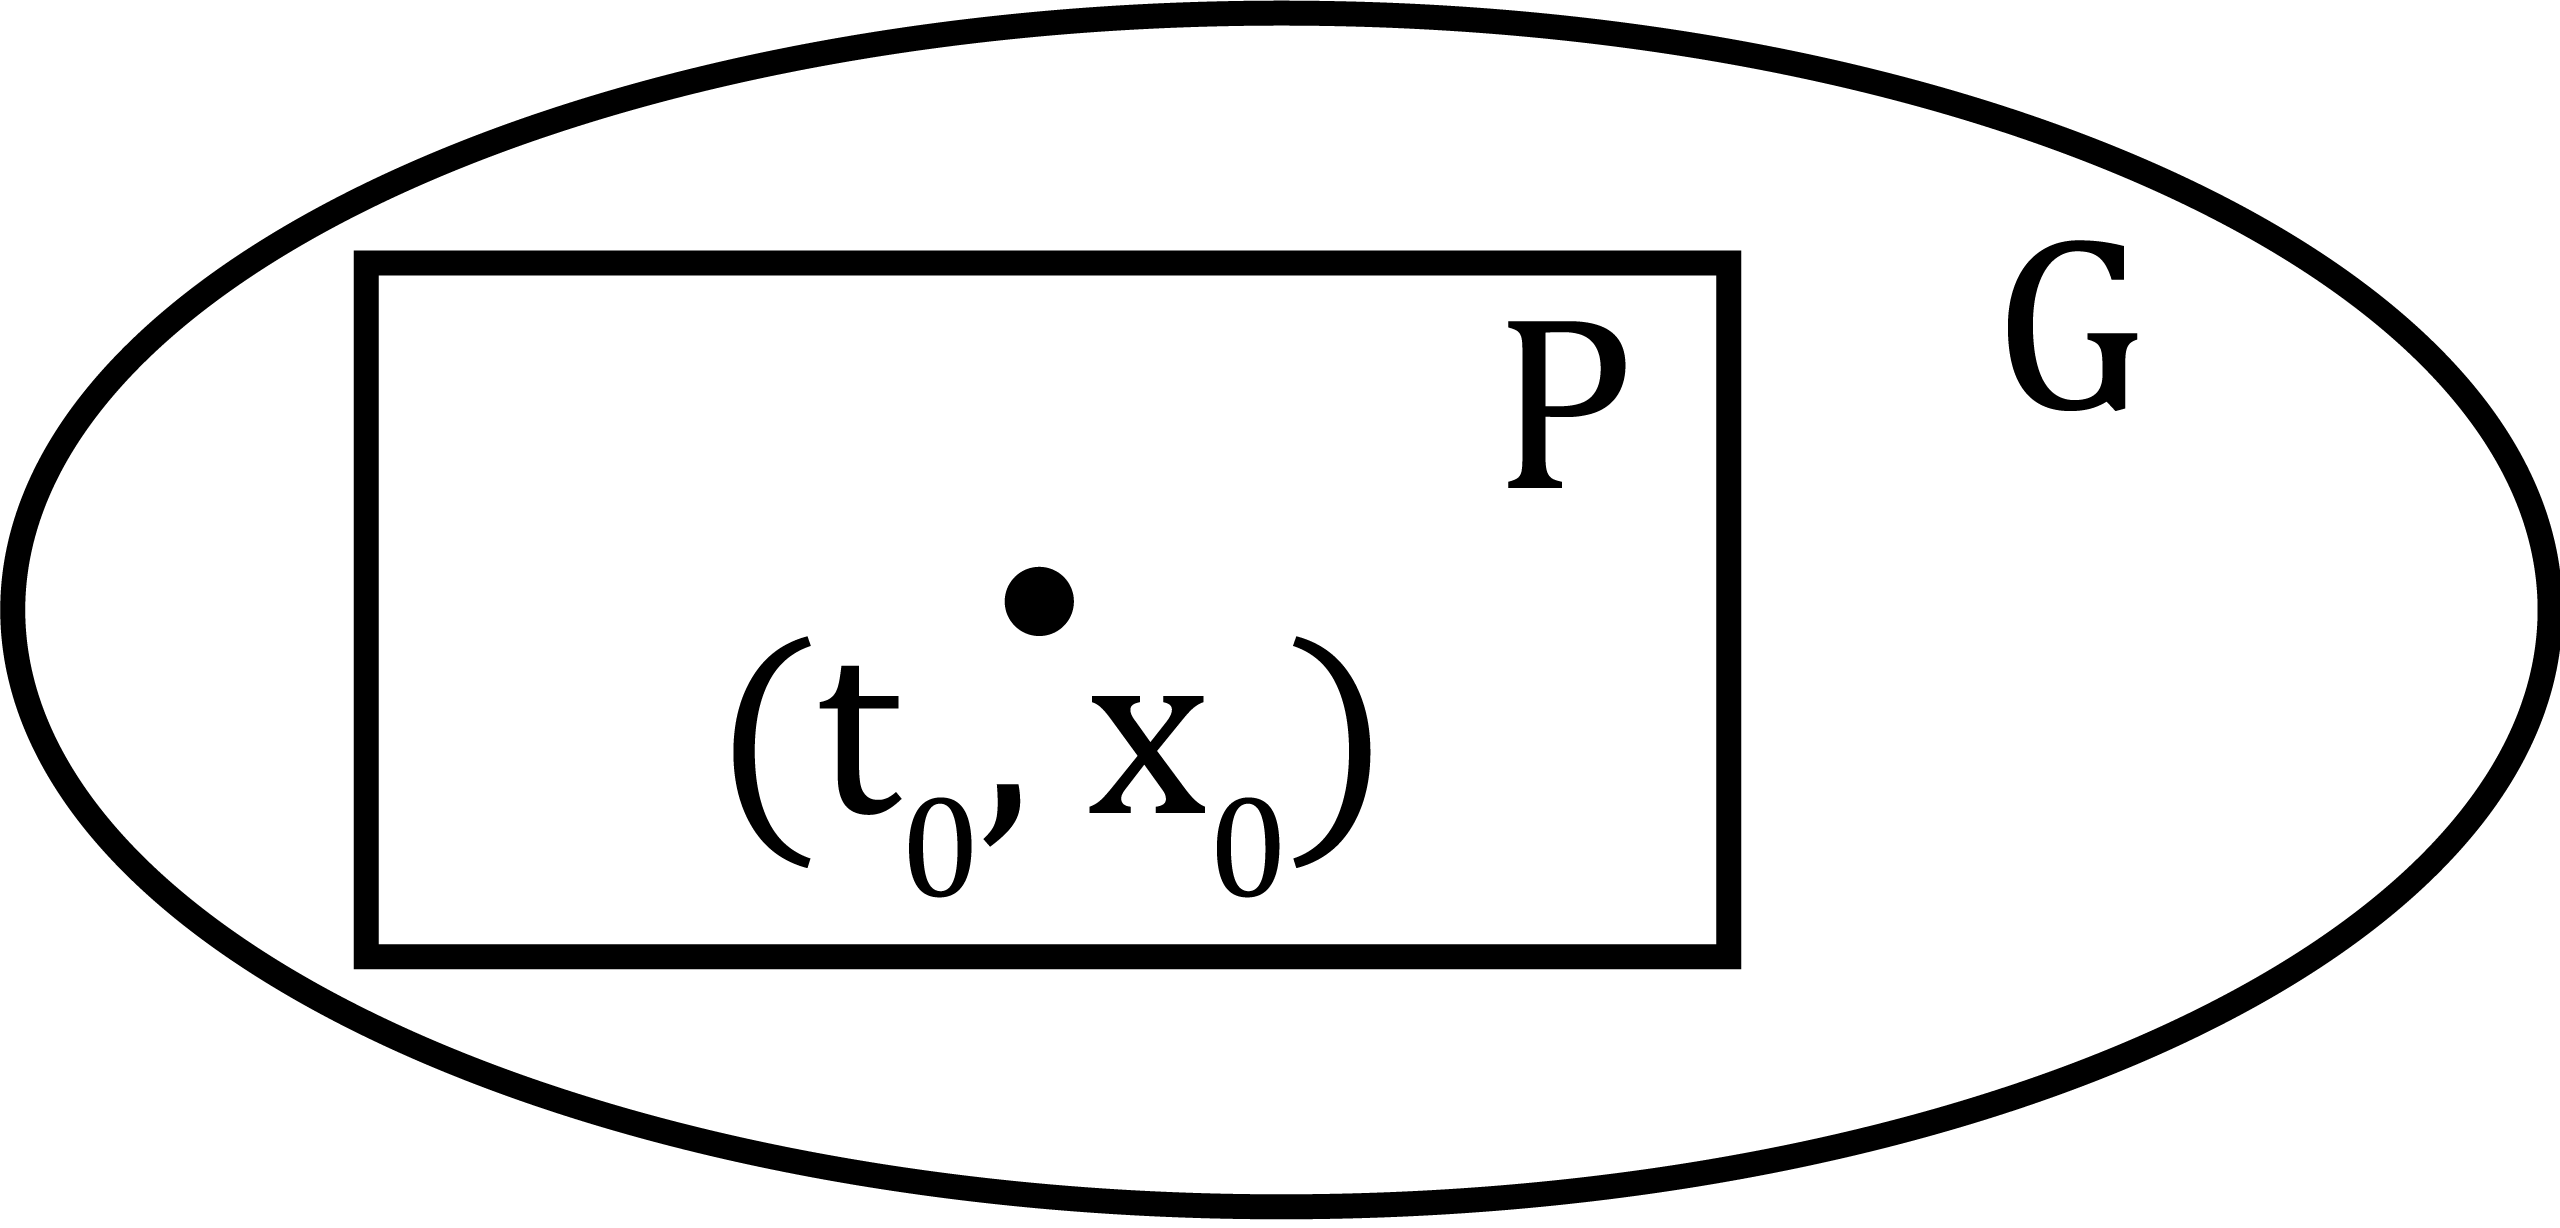
\includegraphics[width=4cm]{pics/3_1.png}
			    	\centering
				\end{figure}
		\end{Proof}

		\begin{Theorem} [единственности]
				\[\dot{x} = \sqrt[3]{x^2} \q\q x \equiv 0 \text{ - реш}\]
				\[x = \left(\frac{t+c}{3}\right)^3\]
				\begin{figure}
						\centering
						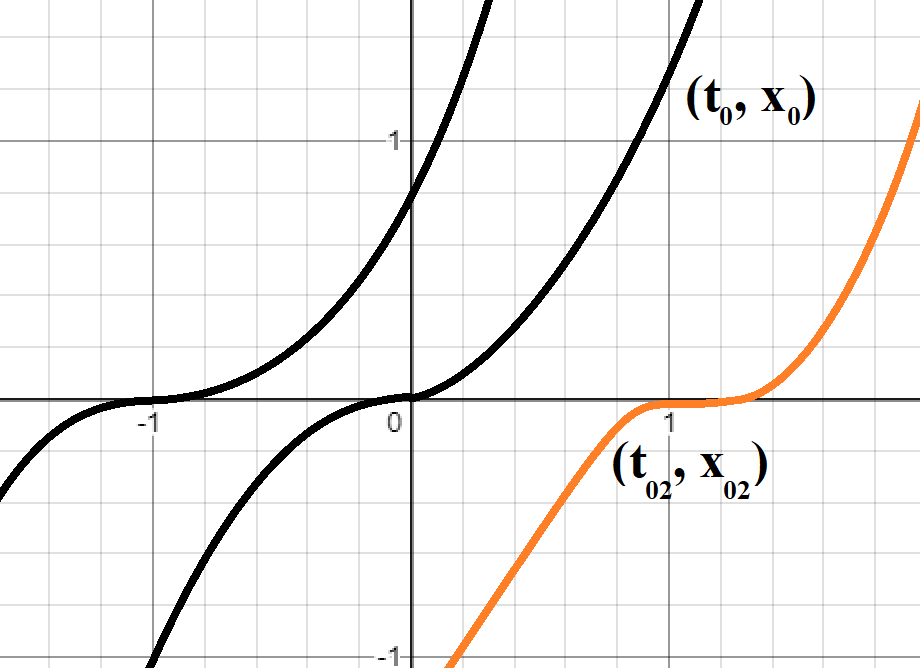
\includegraphics[width=4cm]{pics/3_2.png}
				\end{figure}
				\[\exists \Delta > 0 : \text{ реш } x = \varphi(t) : x_{01} = \varphi(t_{01}) \text{ - единств. на } [t_{01} - \Delta, t_{01} + \Delta]\]
				\[\forall \Delta > 0 \q \text{ через т. } (t_{02}, x_{02}) \text{ проходит беск. много решений}  \]
		\end{Theorem}

		\begin{Definition} [1]
				\[(1) \q \dot{x} = X(t, x) \q X \in C(G) \q \underbracket{G}_{\text{обл}} \subset \R^2 \]
				\[(t_0, x_0) \in G \text{ - точка единств. для } (1) \text{, если}\]
				\[\exists \Delta > 0: \text{ реш }(1) x = \varphi(t) \q (x_0 = \varphi(t_0))\]
				\[\text{опред и единственно на } [t_0 - \Delta, t_0 + \Delta] \text{ вместо отрезка можно взять интервал}\]
		\end{Definition}

		\begin{Definition}[1']
				\[(t_0, x_0) \in G \text{ - точка единств } (1) \text{, если}\]
				\[\exists \Delta > 0 : \forall \delta : 0 < \delta \leq \Delta \text{ реш }\]
				\[x = \varphi(t) \text{ - опред и ед-гл на } (t_0 - \delta, t_0 + \delta)\]
				\[(x_0 = \varphi(t_0))\]
		\end{Definition}

		\begin{Theorem}
				\[\letus \ x = \varphi(t) \text{ - реш. з. К } (1)(2), \text{ опред. при } t \in <a, b>\]
				\[\forall t \in (a, b) \q (t, \varphi(t)) \text{ - точка ед-ти}\]
				\[\Ra \text{ реш } x = \varphi (t) \text{ - ед-но на }<a, b>\]
		\end{Theorem}

		\begin{Proof}
				\[\letus \ \exists x = \psi(t) \text{ - другое. реш. З.К. } (1),(2) \q t \in <a, b>\]
				\[\exists t^* \in (a,b) : \varphi(t^*) \neq \psi(t^*) \q t^*\neq t_0 \q (\text{т.к } \varphi(t_0) = \psi(t_0))\]
				\[\text{НУО } t^* > t_0\]
				\begin{figure}[H]
				    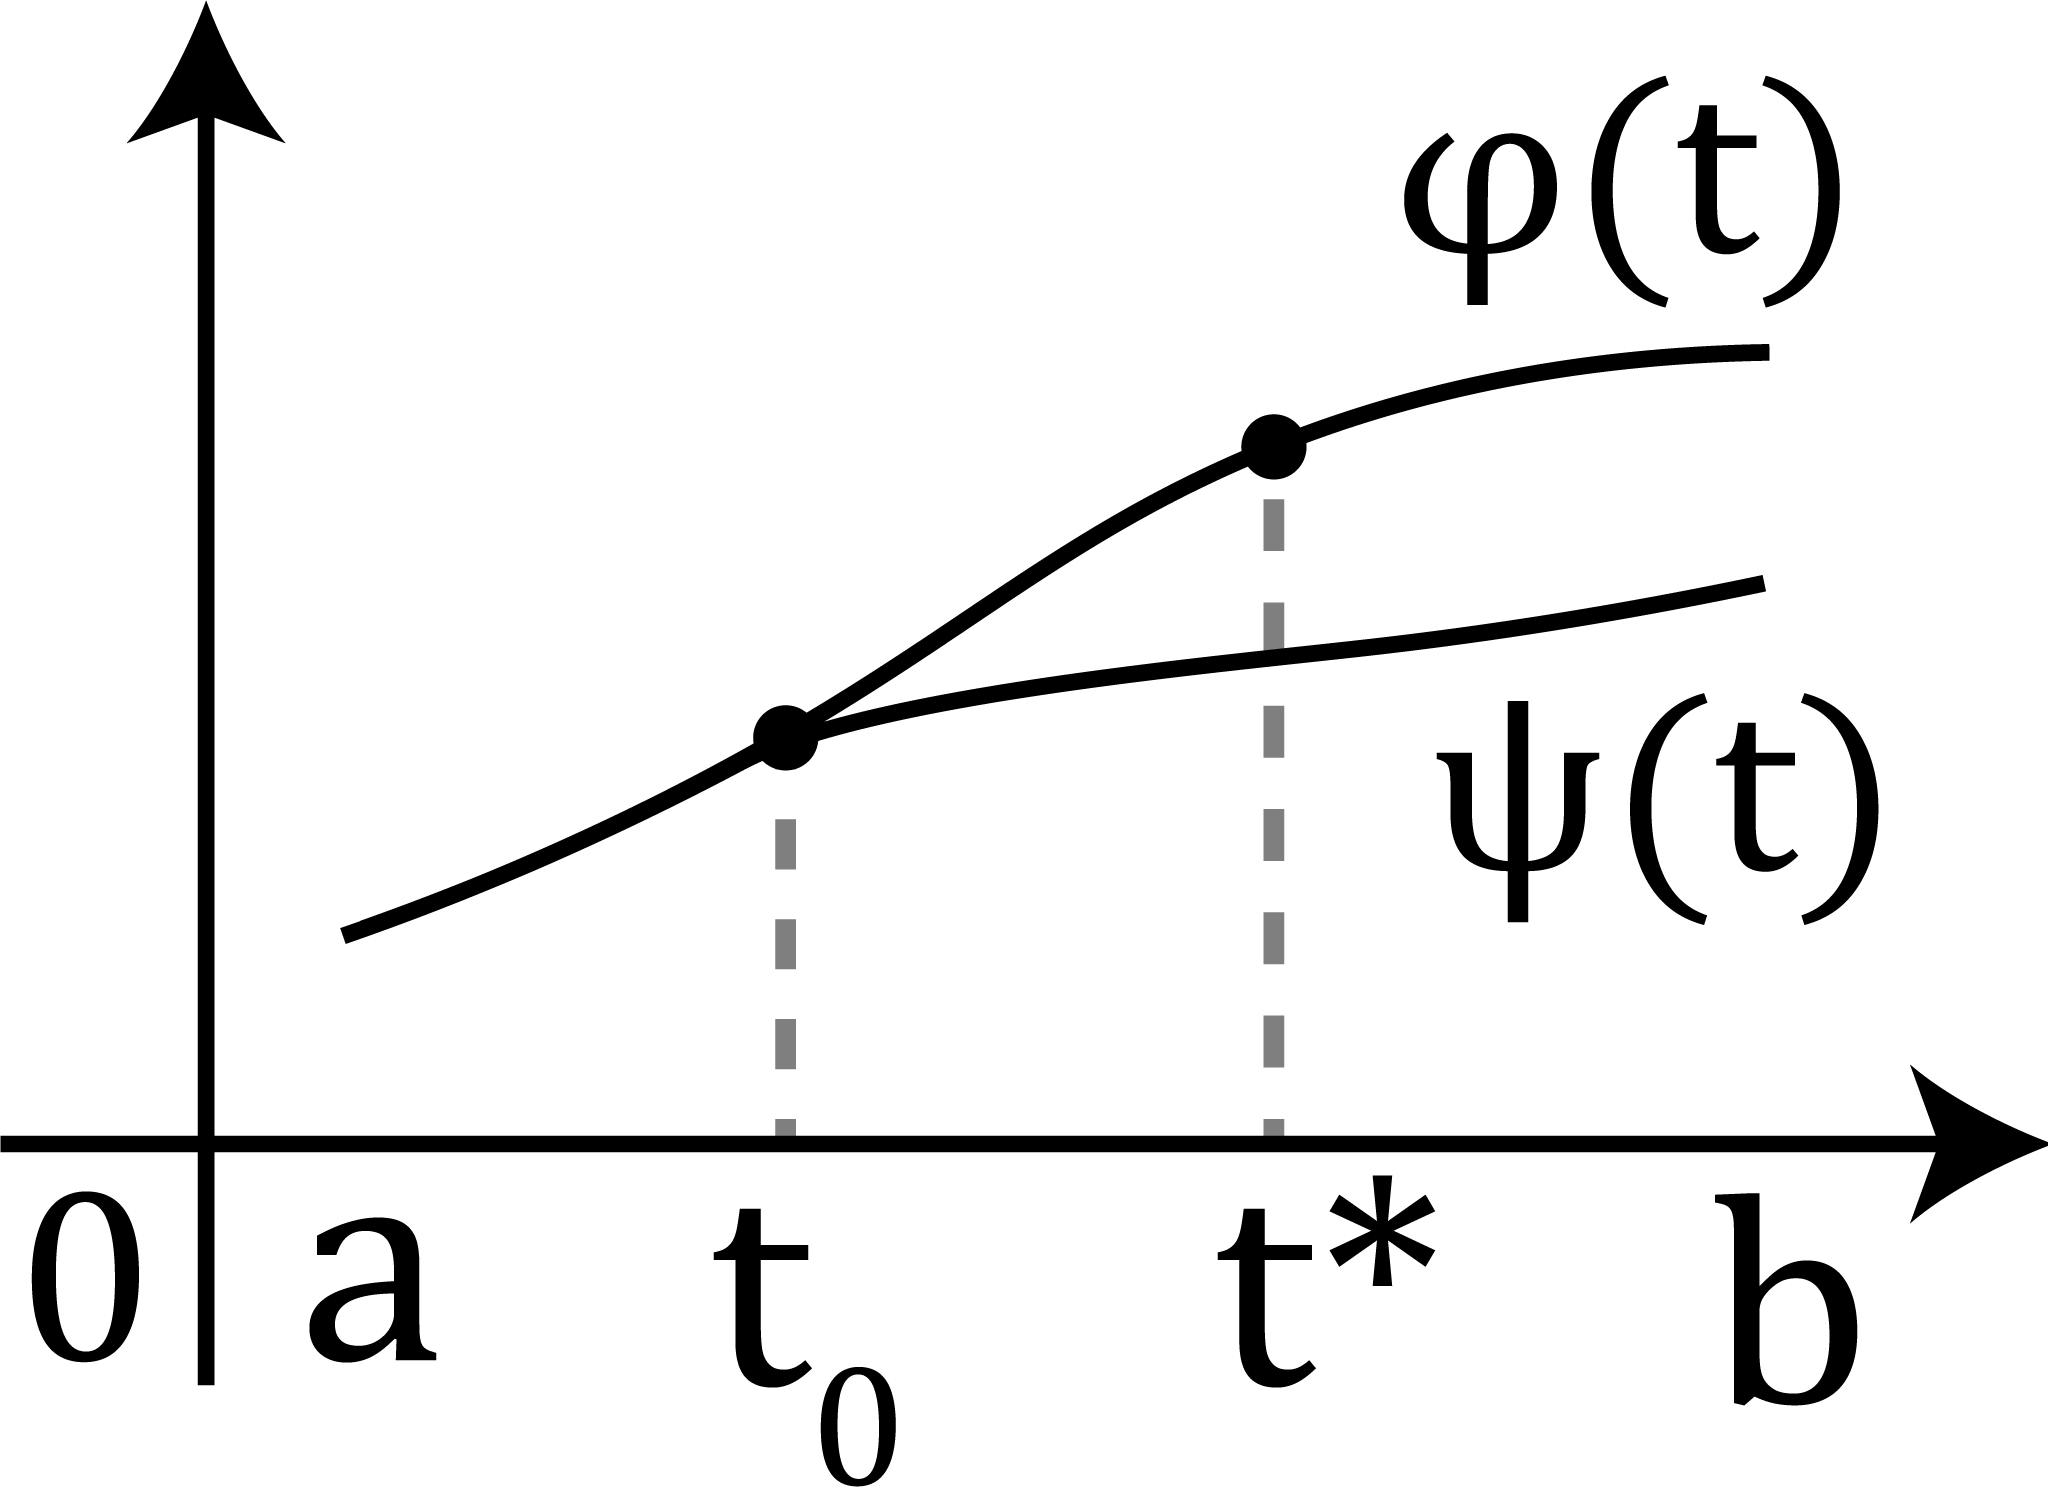
\includegraphics[width=4cm]{pics/3_3.png}
				    \centering
				\end{figure}
				\[u(t) = \varphi(t) - \psi(t)\]
				\[O = \{t \in [t_0, t^*] : u(t) = 0\}\]
				\[O \neq \varnothing \q (t_0 \in O)\]
				\[O \text{ - замкн и огр}\]
				\[\exists t_1 \in [t_0, t^*) : \q t_1 = \max O \q (t_1 \in O)\]
				\[\Ra \varphi(t_1) = \psi(t_1) \q \varphi(t) \neq \psi(t) \q \forall t \in (t_1, t^*]\]
				\[\text{Ставим З.К } (t_1, \varphi(t_1) \q \exists h > 0:\]
				\[\text{На } [t_1 - h, t_1 + h] \text{ опред. реш. } x = \widetilde{\varphi}(t) : \q x_1 = \widetilde{\varphi}(t_1)\]
				\[\exists \Delta > 0 : \q \Delta < \min(h, t_1 - a, t^* - t_1 )\]
				\[(t_1, x_1) \text{ - точка ед-ти } \Ra \exists \Delta < \min(h, t_1 - a, t^* - t_1)\]
				\[\Ra \text{ на } [t_1 - \Delta, t_1 + \Delta] \q \widetilde{\varphi} \equiv \varphi(t) \equiv \psi(t)\]
				противореч с опред $t_1$
		\end{Proof}

		\addcontentsline{toc}{subsection}{Лемма Гронуолла}
		\begin{Lemma} [Гронуолла]
				\[u(t) \geq 0, \text{ опред } t \in <a, b>, \q u(t) \text{ - непр на } <a, b>\]
				\[\exists  t_0 \in (a, b), \q c \geq 0, \q L > 0:\]
				\[u(t) \leq c + L \abs{\int^t_{t_0} u(\tau) d\tau } \q \forall t \in <a, b> \q (3)\]
				\[\Ra u(t) \leq c \cdot e^{L \abs{t - t_0}} \]
		\end{Lemma}

		\begin{Proof}
				\[\text{НУО } t \geq t_0\]
				\[(3') \q u(t) \leq  \underbracket{c + L \int^t_{t_0} u(\tau) d\tau}_{v(t)}
				\os{?}{\Ra} (4') \q u(t) \leq c \cdot e^{L(t - t_0)}  \]
				\[u(t) \leq v(t)\]
				\[\frac{d}{dt}(v(t) \cdot e^{-Lt} ) = \underbracket{\dot{v}(t)}_{L \cdot u(t)}  e^{-Lt} + v(t)(-L) e^{-Lt} =  \]
				\[L \cdot e^{-Lt}(u(t) - v(t)) \leq 0 \]
				\[v(t) e^{-Lt} \text{ - убыв. } \Ra \]
				\[v(t) e^{-Lt} \leq v(t_0) e^{-Lt_0} \Ra \]
				\[U(t) \leq v(t) \leq \underbracket{v(t_0)}_{=c} \cdot e^{L(t-t_0)} = c \cdot e ^{L(t-t_0)}   \]
		\end{Proof}

		\begin{Consequence}
				\[\text{Если } c = 0, \text{ то } u(t) \equiv 0 \text{ на } <a, b>\]
		\end{Consequence}
\end{lect}
\end{document}
